% NJ-0502 --- Atividade 06, item 2
% Arquivo unico para o relatorio: % NJ-0502 --- Atividade 06, item 2
% Arquivo unico para o relatorio: % NJ-0502 --- Atividade 06, item 2
% Arquivo unico para o relatorio: % NJ-0502 --- Atividade 06, item 2
% Arquivo unico para o relatorio: \input{item2_resultados}
% Copie tambem resultados_q2/cl_cm_asa.png para o Overleaf.
\graphicspath{{../resultados_q2/}{./}}

Condição: $V_A$, $n_z = 2{,}5$, CG dianteiro (\texttt{fwd.avl}, washout $-7^\circ$), aeronave trimada ($C_M = 0$) e com taxa de arfagem $q = g(n_z-1)/V_{\mathrm{TAS}}$. O $C_L$ imposto no AVL é o $C_{L_{\max}}$ do designTool ($0{,}9\,c_{\ell,\max}\cos\Lambda = 1{,}304$).

\begin{table}[htbp]
\centering
\caption{Pesos na condição de manobra ($V_A$, $n_{\max}$).}
\label{tab:q2-pesos}
\begin{tabular}{lrr}
\toprule
 & Início do cruzeiro & Fim do cruzeiro \\
\midrule
Peso da aeronave & $261\,172$ kgf ($2\,562\,102$ N) & $182\,623$ kgf ($1\,791\,530$ N) \\
Peso da asa & $36\,148$ kgf ($354\,617$ N) & $36\,148$ kgf ($354\,617$ N) \\
Peso do combustível & $85\,870$ kgf ($842\,383$ N) & $7\,320$ kgf ($71\,811$ N) \\
Peso de cada MLG & $4\,994$ kgf ($48\,993$ N) & $4\,994$ kgf ($48\,993$ N) \\
Peso de cada motor (instalado) & $9\,463$ kgf ($92\,835$ N) & $9\,463$ kgf ($92\,835$ N) \\
\bottomrule
\end{tabular}
\end{table}

\begin{table}[htbp]
\centering
\caption{Condição de voo e solução do AVL em $V_A$.}
\label{tab:q2-voo}
\begin{tabular}{lrr}
\toprule
 & Início do cruzeiro & Fim do cruzeiro \\
\midrule
$V_A$ (EAS) [m/s] & $144{,}7$ & $121{,}0$ \\
$V_A$ (TAS) [m/s] & $259{,}7$ & $217{,}1$ \\
Mach & $0{,}876$ & $0{,}732$ \\
$n_z$ & $2{,}5$ & $2{,}5$ \\
$C_L$ (alvo / AVL) & $1{,}304$ / $1{,}304$ & $1{,}304$ / $1{,}304$ \\
$\alpha$ da fuselagem [$^\circ$] & $9{,}19$ & $10{,}80$ \\
$i_t$ [$^\circ$] & $-1{,}143$ & $-1{,}143$ \\
$\delta_e$ [$^\circ$] & $-5{,}23$ & $-6{,}49$ \\
$C_M$ & $0{,}000$ & $0{,}000$ \\
$q$ [rad/s] & $0{,}0567$ & $0{,}0678$ \\
$qc/2V$ (pedido / AVL) & $0{,}00075$ / $0{,}00075$ & $0{,}00108$ / $0{,}00108$ \\
\bottomrule
\end{tabular}
\end{table}

\begin{table}[htbp]
\centering
\caption{Forças de sustentação em $V_A$, $n_z = 2{,}5$.}
\label{tab:q2-forcas}
\begin{tabular}{lrr}
\toprule
 & Início do cruzeiro & Fim do cruzeiro \\
\midrule
Sustentação da asa & $625\,480$ kgf ($6\,135\,961$ N) & $431\,631$ kgf ($4\,234\,298$ N) \\
Sustentação da EH & $2\,167$ kgf ($21\,261$ N) & $4\,772$ kgf ($46\,809$ N) \\
$n_z W$ & $652\,931$ kgf ($6\,405\,254$ N) & $456\,557$ kgf ($4\,478\,824$ N) \\
$C_L\,q_\infty S$ & $652\,930$ kgf ($6\,405\,239$ N) & $456\,556$ kgf ($4\,478\,813$ N) \\
\bottomrule
\end{tabular}
\end{table}

\begin{figure}[htbp]
\centering
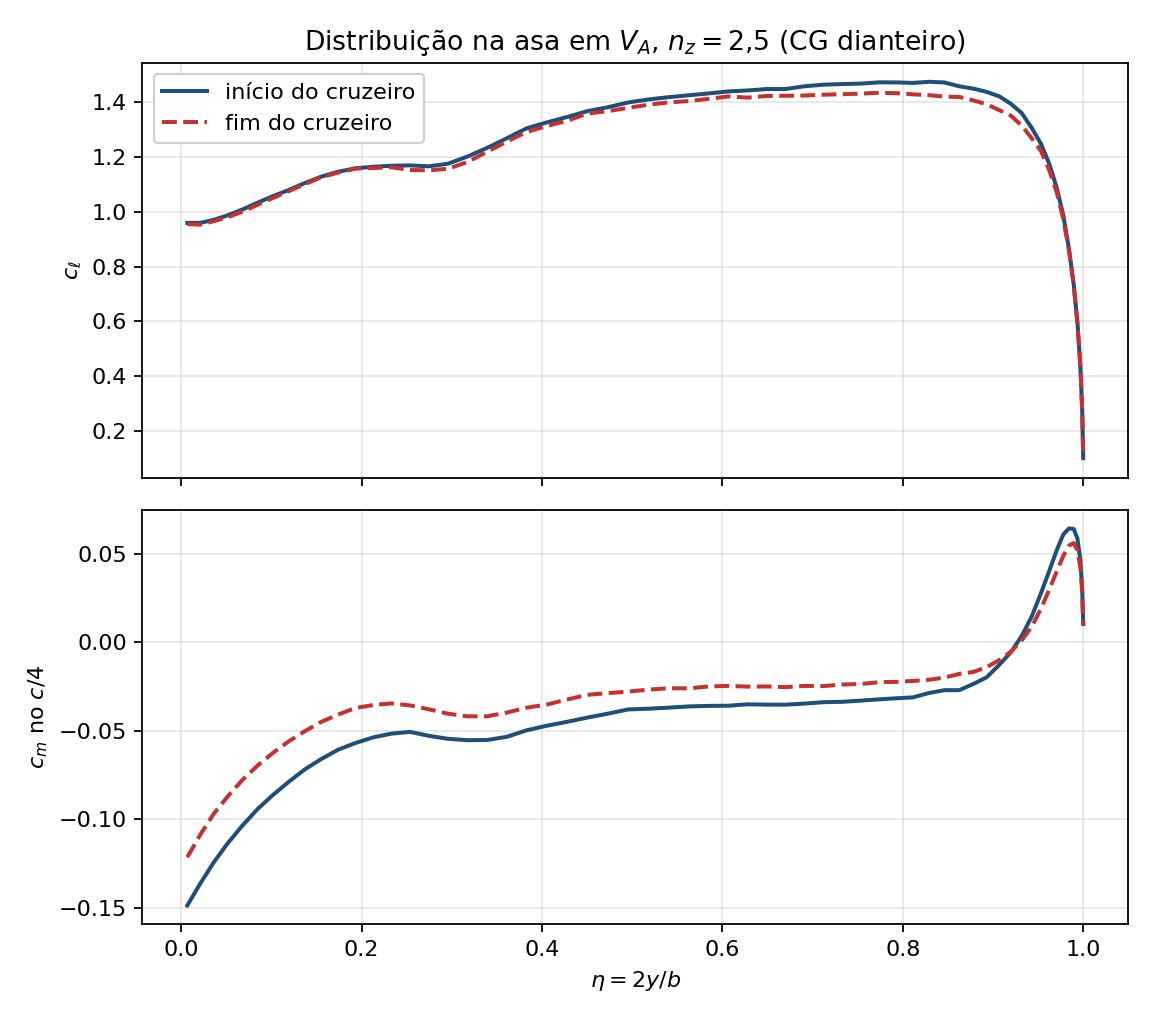
\includegraphics[width=0.92\textwidth]{cl_cm_asa.png}
\caption{Distribuição de $c_\ell$ e de $c_m$ no $c/4$ ao longo da asa em $V_A$, $n_z = 2{,}5$ (CG dianteiro).}
\label{fig:q2-cl-cm}
\end{figure}

As duas condições impõem o mesmo $C_L = C_{L_{\max}}$, por isso as curvas de $c_\ell$ quase coincidem. O $\alpha$ maior no fim do cruzeiro ($10{,}80^\circ$ contra $9{,}19^\circ$) acompanha o Mach menor ($0{,}732$ contra $0{,}876$). O profundor fica a $-5{,}2^\circ$ e $-6{,}5^\circ$, e $C_L q_\infty S$ fecha com $n_z W$. A EH sustenta pouco e para cima: com $\alpha \approx 9$--$11^\circ$, o $i_t = -1{,}143^\circ$ não chega a gerar download. O $c_\ell$ sobe da raiz ($\approx 0{,}96$) até um platô $\approx 1{,}47$ em $\eta \approx 0{,}75$--$0{,}85$ e cai na ponta; o $c_m$ no $c/4$ é picado na raiz. Pelo critério da seção crítica do Lab~04 ($c_{\ell,\mathrm{norm}}/c_{\ell,\max}$), várias seções externas já estariam além do teto 2D --- o AVL não estola e entrega a carga potencial pedida no enunciado. O pico de $c_m$ positivo em $\eta > 0{,}92$ é artefato de ponta da treliça de vórtices.


% Copie tambem resultados_q2/cl_cm_asa.png para o Overleaf.
\graphicspath{{../resultados_q2/}{./}}

Condição: $V_A$, $n_z = 2{,}5$, CG dianteiro (\texttt{fwd.avl}, washout $-7^\circ$), aeronave trimada ($C_M = 0$) e com taxa de arfagem $q = g(n_z-1)/V_{\mathrm{TAS}}$. O $C_L$ imposto no AVL é o $C_{L_{\max}}$ do designTool ($0{,}9\,c_{\ell,\max}\cos\Lambda = 1{,}304$).

\begin{table}[htbp]
\centering
\caption{Pesos na condição de manobra ($V_A$, $n_{\max}$).}
\label{tab:q2-pesos}
\begin{tabular}{lrr}
\toprule
 & Início do cruzeiro & Fim do cruzeiro \\
\midrule
Peso da aeronave & $261\,172$ kgf ($2\,562\,102$ N) & $182\,623$ kgf ($1\,791\,530$ N) \\
Peso da asa & $36\,148$ kgf ($354\,617$ N) & $36\,148$ kgf ($354\,617$ N) \\
Peso do combustível & $85\,870$ kgf ($842\,383$ N) & $7\,320$ kgf ($71\,811$ N) \\
Peso de cada MLG & $4\,994$ kgf ($48\,993$ N) & $4\,994$ kgf ($48\,993$ N) \\
Peso de cada motor (instalado) & $9\,463$ kgf ($92\,835$ N) & $9\,463$ kgf ($92\,835$ N) \\
\bottomrule
\end{tabular}
\end{table}

\begin{table}[htbp]
\centering
\caption{Condição de voo e solução do AVL em $V_A$.}
\label{tab:q2-voo}
\begin{tabular}{lrr}
\toprule
 & Início do cruzeiro & Fim do cruzeiro \\
\midrule
$V_A$ (EAS) [m/s] & $144{,}7$ & $121{,}0$ \\
$V_A$ (TAS) [m/s] & $259{,}7$ & $217{,}1$ \\
Mach & $0{,}876$ & $0{,}732$ \\
$n_z$ & $2{,}5$ & $2{,}5$ \\
$C_L$ (alvo / AVL) & $1{,}304$ / $1{,}304$ & $1{,}304$ / $1{,}304$ \\
$\alpha$ da fuselagem [$^\circ$] & $9{,}19$ & $10{,}80$ \\
$i_t$ [$^\circ$] & $-1{,}143$ & $-1{,}143$ \\
$\delta_e$ [$^\circ$] & $-5{,}23$ & $-6{,}49$ \\
$C_M$ & $0{,}000$ & $0{,}000$ \\
$q$ [rad/s] & $0{,}0567$ & $0{,}0678$ \\
$qc/2V$ (pedido / AVL) & $0{,}00075$ / $0{,}00075$ & $0{,}00108$ / $0{,}00108$ \\
\bottomrule
\end{tabular}
\end{table}

\begin{table}[htbp]
\centering
\caption{Forças de sustentação em $V_A$, $n_z = 2{,}5$.}
\label{tab:q2-forcas}
\begin{tabular}{lrr}
\toprule
 & Início do cruzeiro & Fim do cruzeiro \\
\midrule
Sustentação da asa & $625\,480$ kgf ($6\,135\,961$ N) & $431\,631$ kgf ($4\,234\,298$ N) \\
Sustentação da EH & $2\,167$ kgf ($21\,261$ N) & $4\,772$ kgf ($46\,809$ N) \\
$n_z W$ & $652\,931$ kgf ($6\,405\,254$ N) & $456\,557$ kgf ($4\,478\,824$ N) \\
$C_L\,q_\infty S$ & $652\,930$ kgf ($6\,405\,239$ N) & $456\,556$ kgf ($4\,478\,813$ N) \\
\bottomrule
\end{tabular}
\end{table}

\begin{figure}[htbp]
\centering
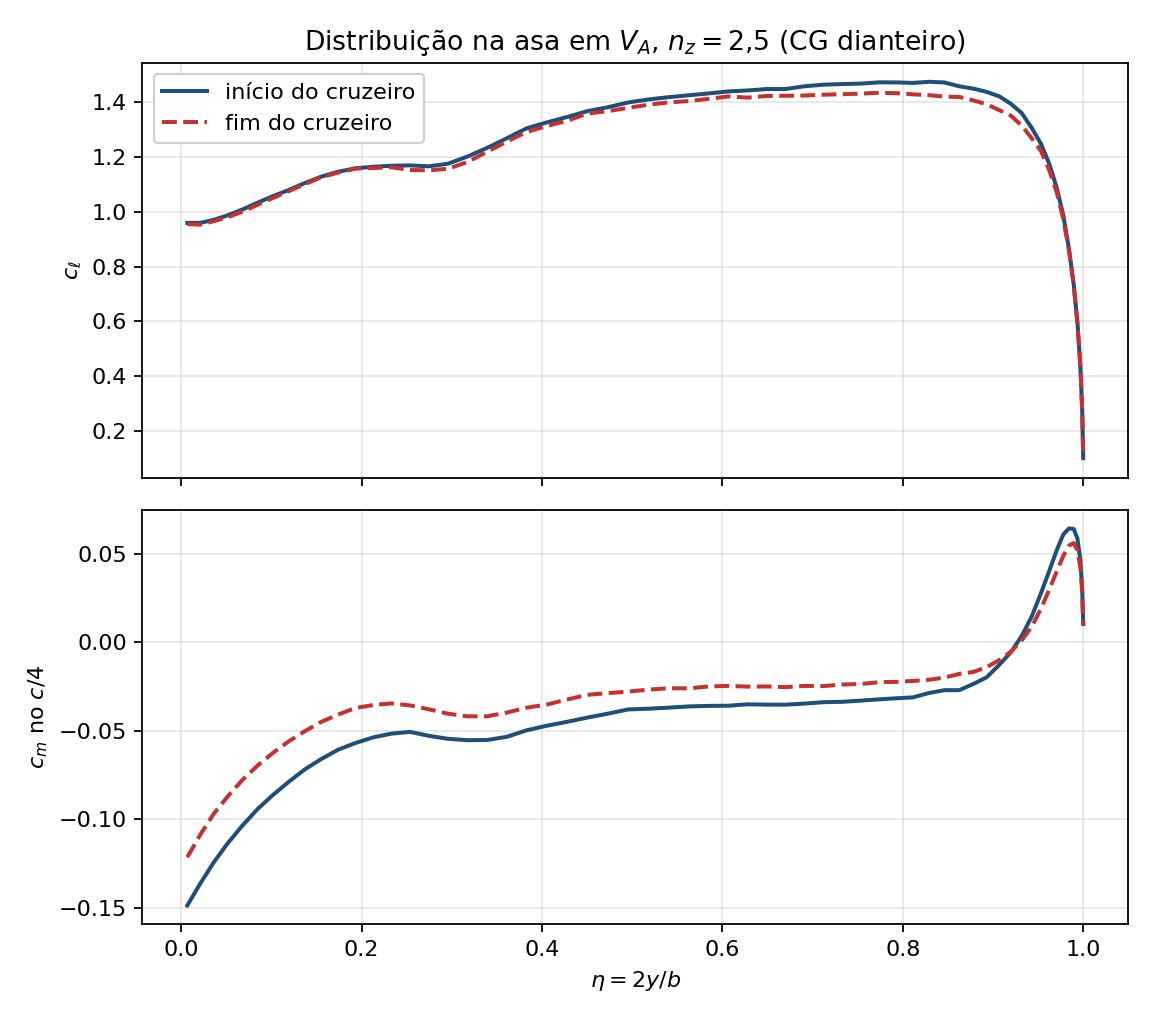
\includegraphics[width=0.92\textwidth]{cl_cm_asa.png}
\caption{Distribuição de $c_\ell$ e de $c_m$ no $c/4$ ao longo da asa em $V_A$, $n_z = 2{,}5$ (CG dianteiro).}
\label{fig:q2-cl-cm}
\end{figure}

As duas condições impõem o mesmo $C_L = C_{L_{\max}}$, por isso as curvas de $c_\ell$ quase coincidem. O $\alpha$ maior no fim do cruzeiro ($10{,}80^\circ$ contra $9{,}19^\circ$) acompanha o Mach menor ($0{,}732$ contra $0{,}876$). O profundor fica a $-5{,}2^\circ$ e $-6{,}5^\circ$, e $C_L q_\infty S$ fecha com $n_z W$. A EH sustenta pouco e para cima: com $\alpha \approx 9$--$11^\circ$, o $i_t = -1{,}143^\circ$ não chega a gerar download. O $c_\ell$ sobe da raiz ($\approx 0{,}96$) até um platô $\approx 1{,}47$ em $\eta \approx 0{,}75$--$0{,}85$ e cai na ponta; o $c_m$ no $c/4$ é picado na raiz. Pelo critério da seção crítica do Lab~04 ($c_{\ell,\mathrm{norm}}/c_{\ell,\max}$), várias seções externas já estariam além do teto 2D --- o AVL não estola e entrega a carga potencial pedida no enunciado. O pico de $c_m$ positivo em $\eta > 0{,}92$ é artefato de ponta da treliça de vórtices.


% Copie tambem resultados_q2/cl_cm_asa.png para o Overleaf.
\graphicspath{{../resultados_q2/}{./}}

Condição: $V_A$, $n_z = 2{,}5$, CG dianteiro (\texttt{fwd.avl}, washout $-7^\circ$), aeronave trimada ($C_M = 0$) e com taxa de arfagem $q = g(n_z-1)/V_{\mathrm{TAS}}$. O $C_L$ imposto no AVL é o $C_{L_{\max}}$ do designTool ($0{,}9\,c_{\ell,\max}\cos\Lambda = 1{,}304$).

\begin{table}[htbp]
\centering
\caption{Pesos na condição de manobra ($V_A$, $n_{\max}$).}
\label{tab:q2-pesos}
\begin{tabular}{lrr}
\toprule
 & Início do cruzeiro & Fim do cruzeiro \\
\midrule
Peso da aeronave & $261\,172$ kgf ($2\,562\,102$ N) & $182\,623$ kgf ($1\,791\,530$ N) \\
Peso da asa & $36\,148$ kgf ($354\,617$ N) & $36\,148$ kgf ($354\,617$ N) \\
Peso do combustível & $85\,870$ kgf ($842\,383$ N) & $7\,320$ kgf ($71\,811$ N) \\
Peso de cada MLG & $4\,994$ kgf ($48\,993$ N) & $4\,994$ kgf ($48\,993$ N) \\
Peso de cada motor (instalado) & $9\,463$ kgf ($92\,835$ N) & $9\,463$ kgf ($92\,835$ N) \\
\bottomrule
\end{tabular}
\end{table}

\begin{table}[htbp]
\centering
\caption{Condição de voo e solução do AVL em $V_A$.}
\label{tab:q2-voo}
\begin{tabular}{lrr}
\toprule
 & Início do cruzeiro & Fim do cruzeiro \\
\midrule
$V_A$ (EAS) [m/s] & $144{,}7$ & $121{,}0$ \\
$V_A$ (TAS) [m/s] & $259{,}7$ & $217{,}1$ \\
Mach & $0{,}876$ & $0{,}732$ \\
$n_z$ & $2{,}5$ & $2{,}5$ \\
$C_L$ (alvo / AVL) & $1{,}304$ / $1{,}304$ & $1{,}304$ / $1{,}304$ \\
$\alpha$ da fuselagem [$^\circ$] & $9{,}19$ & $10{,}80$ \\
$i_t$ [$^\circ$] & $-1{,}143$ & $-1{,}143$ \\
$\delta_e$ [$^\circ$] & $-5{,}23$ & $-6{,}49$ \\
$C_M$ & $0{,}000$ & $0{,}000$ \\
$q$ [rad/s] & $0{,}0567$ & $0{,}0678$ \\
$qc/2V$ (pedido / AVL) & $0{,}00075$ / $0{,}00075$ & $0{,}00108$ / $0{,}00108$ \\
\bottomrule
\end{tabular}
\end{table}

\begin{table}[htbp]
\centering
\caption{Forças de sustentação em $V_A$, $n_z = 2{,}5$.}
\label{tab:q2-forcas}
\begin{tabular}{lrr}
\toprule
 & Início do cruzeiro & Fim do cruzeiro \\
\midrule
Sustentação da asa & $625\,480$ kgf ($6\,135\,961$ N) & $431\,631$ kgf ($4\,234\,298$ N) \\
Sustentação da EH & $2\,167$ kgf ($21\,261$ N) & $4\,772$ kgf ($46\,809$ N) \\
$n_z W$ & $652\,931$ kgf ($6\,405\,254$ N) & $456\,557$ kgf ($4\,478\,824$ N) \\
$C_L\,q_\infty S$ & $652\,930$ kgf ($6\,405\,239$ N) & $456\,556$ kgf ($4\,478\,813$ N) \\
\bottomrule
\end{tabular}
\end{table}

\begin{figure}[htbp]
\centering
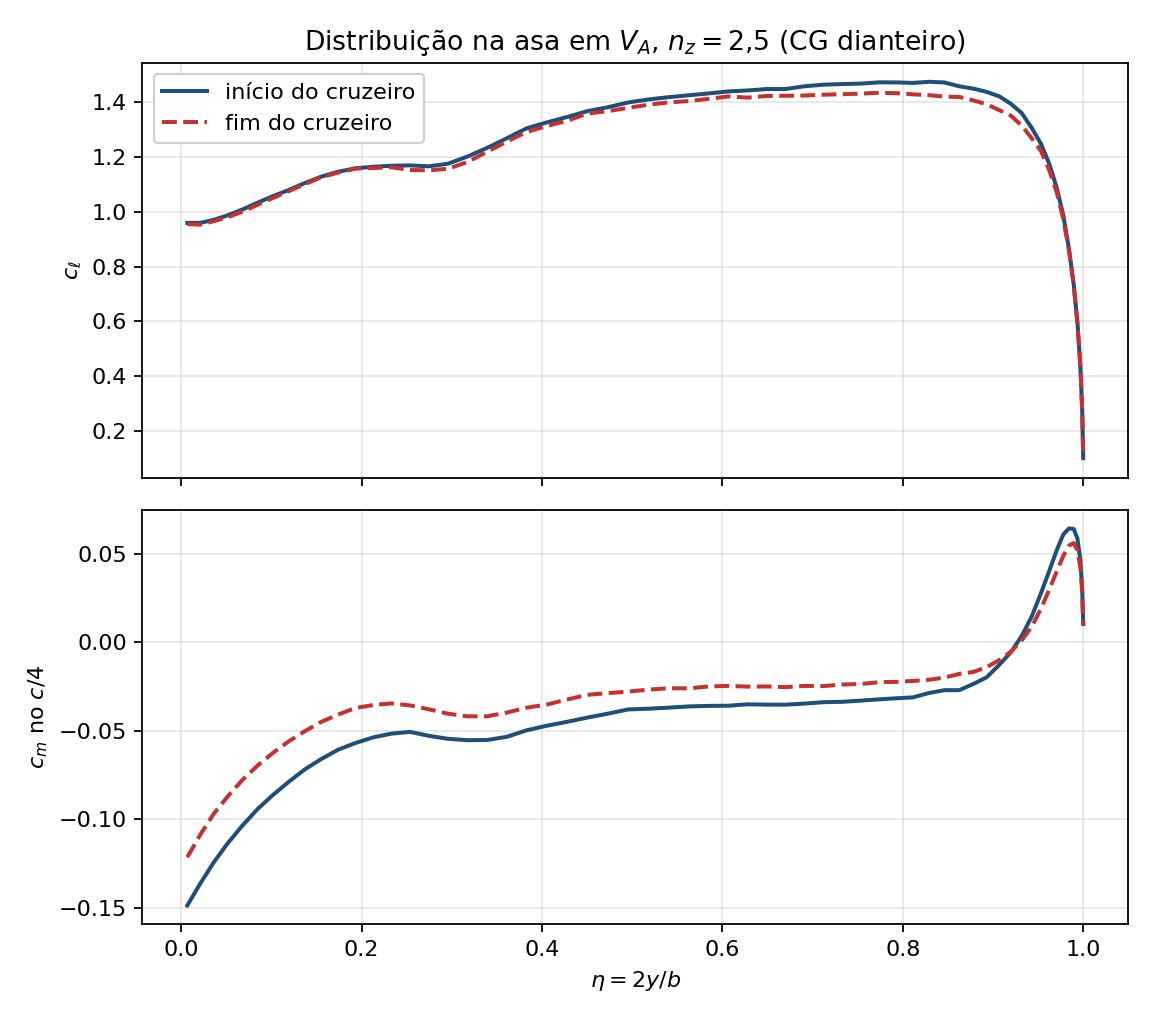
\includegraphics[width=0.92\textwidth]{cl_cm_asa.png}
\caption{Distribuição de $c_\ell$ e de $c_m$ no $c/4$ ao longo da asa em $V_A$, $n_z = 2{,}5$ (CG dianteiro).}
\label{fig:q2-cl-cm}
\end{figure}

As duas condições impõem o mesmo $C_L = C_{L_{\max}}$, por isso as curvas de $c_\ell$ quase coincidem. O $\alpha$ maior no fim do cruzeiro ($10{,}80^\circ$ contra $9{,}19^\circ$) acompanha o Mach menor ($0{,}732$ contra $0{,}876$). O profundor fica a $-5{,}2^\circ$ e $-6{,}5^\circ$, e $C_L q_\infty S$ fecha com $n_z W$. A EH sustenta pouco e para cima: com $\alpha \approx 9$--$11^\circ$, o $i_t = -1{,}143^\circ$ não chega a gerar download. O $c_\ell$ sobe da raiz ($\approx 0{,}96$) até um platô $\approx 1{,}47$ em $\eta \approx 0{,}75$--$0{,}85$ e cai na ponta; o $c_m$ no $c/4$ é picado na raiz. Pelo critério da seção crítica do Lab~04 ($c_{\ell,\mathrm{norm}}/c_{\ell,\max}$), várias seções externas já estariam além do teto 2D --- o AVL não estola e entrega a carga potencial pedida no enunciado. O pico de $c_m$ positivo em $\eta > 0{,}92$ é artefato de ponta da treliça de vórtices.


% Copie tambem resultados_q2/cl_cm_asa.png para o Overleaf.
\graphicspath{{../resultados_q2/}{./}}

Condição: $V_A$, $n_z = 2{,}5$, CG dianteiro (\texttt{fwd.avl}, washout $-7^\circ$), aeronave trimada ($C_M = 0$) e com taxa de arfagem $q = g(n_z-1)/V_{\mathrm{TAS}}$. O $C_L$ imposto no AVL é o $C_{L_{\max}}$ do designTool ($0{,}9\,c_{\ell,\max}\cos\Lambda = 1{,}304$).

\begin{table}[htbp]
\centering
\caption{Pesos na condição de manobra ($V_A$, $n_{\max}$).}
\label{tab:q2-pesos}
\begin{tabular}{lrr}
\toprule
 & Início do cruzeiro & Fim do cruzeiro \\
\midrule
Peso da aeronave & $261\,172$ kgf ($2\,562\,102$ N) & $182\,623$ kgf ($1\,791\,530$ N) \\
Peso da asa & $36\,148$ kgf ($354\,617$ N) & $36\,148$ kgf ($354\,617$ N) \\
Peso do combustível & $85\,870$ kgf ($842\,383$ N) & $7\,320$ kgf ($71\,811$ N) \\
Peso de cada MLG & $4\,994$ kgf ($48\,993$ N) & $4\,994$ kgf ($48\,993$ N) \\
Peso de cada motor (instalado) & $9\,463$ kgf ($92\,835$ N) & $9\,463$ kgf ($92\,835$ N) \\
\bottomrule
\end{tabular}
\end{table}

\begin{table}[htbp]
\centering
\caption{Condição de voo e solução do AVL em $V_A$.}
\label{tab:q2-voo}
\begin{tabular}{lrr}
\toprule
 & Início do cruzeiro & Fim do cruzeiro \\
\midrule
$V_A$ (EAS) [m/s] & $144{,}7$ & $121{,}0$ \\
$V_A$ (TAS) [m/s] & $259{,}7$ & $217{,}1$ \\
Mach & $0{,}876$ & $0{,}732$ \\
$n_z$ & $2{,}5$ & $2{,}5$ \\
$C_L$ (alvo / AVL) & $1{,}304$ / $1{,}304$ & $1{,}304$ / $1{,}304$ \\
$\alpha$ da fuselagem [$^\circ$] & $9{,}19$ & $10{,}80$ \\
$i_t$ [$^\circ$] & $-1{,}143$ & $-1{,}143$ \\
$\delta_e$ [$^\circ$] & $-5{,}23$ & $-6{,}49$ \\
$C_M$ & $0{,}000$ & $0{,}000$ \\
$q$ [rad/s] & $0{,}0567$ & $0{,}0678$ \\
$qc/2V$ (pedido / AVL) & $0{,}00075$ / $0{,}00075$ & $0{,}00108$ / $0{,}00108$ \\
\bottomrule
\end{tabular}
\end{table}

\begin{table}[htbp]
\centering
\caption{Forças de sustentação em $V_A$, $n_z = 2{,}5$.}
\label{tab:q2-forcas}
\begin{tabular}{lrr}
\toprule
 & Início do cruzeiro & Fim do cruzeiro \\
\midrule
Sustentação da asa & $625\,480$ kgf ($6\,135\,961$ N) & $431\,631$ kgf ($4\,234\,298$ N) \\
Sustentação da EH & $2\,167$ kgf ($21\,261$ N) & $4\,772$ kgf ($46\,809$ N) \\
$n_z W$ & $652\,931$ kgf ($6\,405\,254$ N) & $456\,557$ kgf ($4\,478\,824$ N) \\
$C_L\,q_\infty S$ & $652\,930$ kgf ($6\,405\,239$ N) & $456\,556$ kgf ($4\,478\,813$ N) \\
\bottomrule
\end{tabular}
\end{table}

\begin{figure}[htbp]
\centering
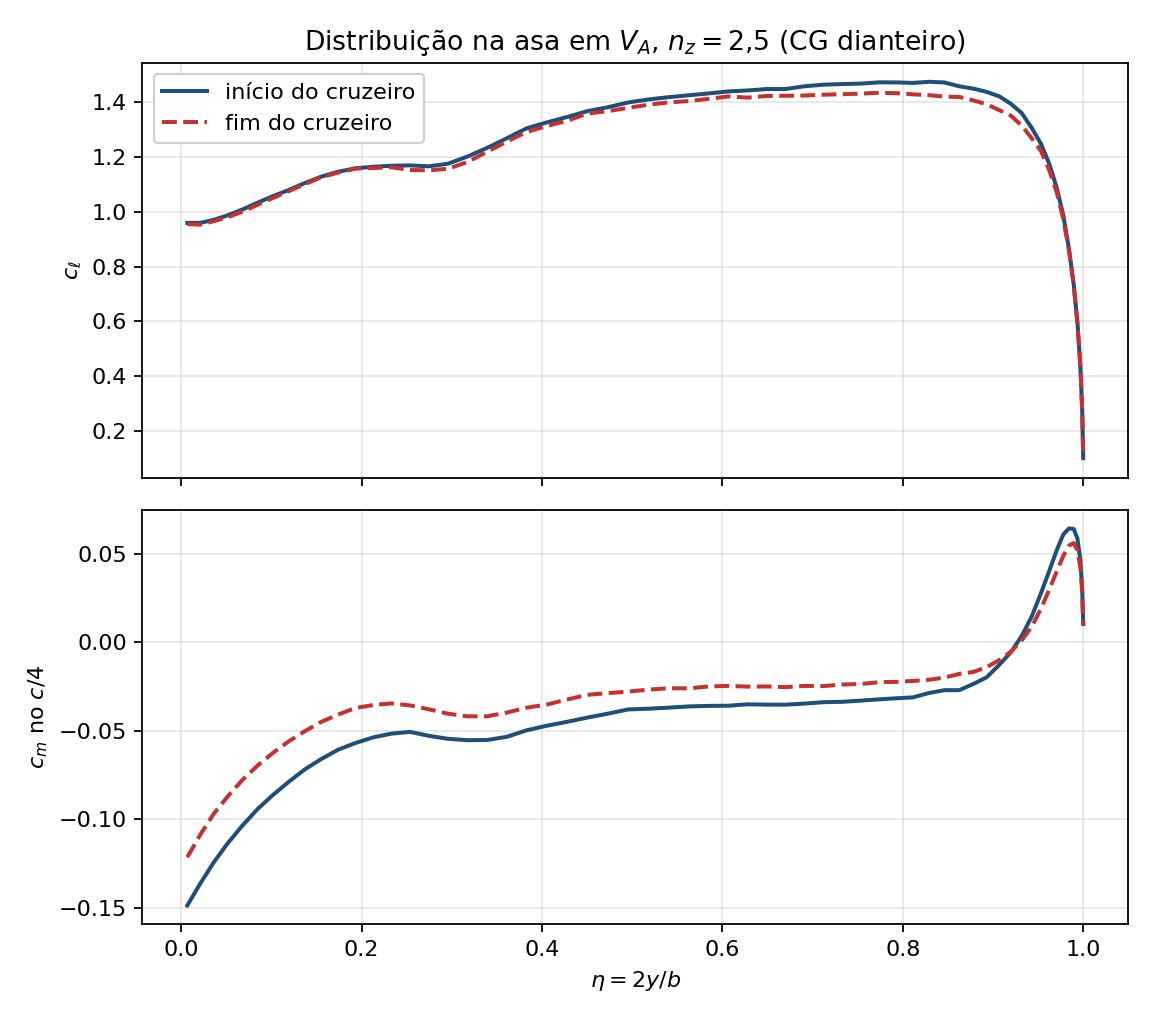
\includegraphics[width=0.92\textwidth]{cl_cm_asa.png}
\caption{Distribuição de $c_\ell$ e de $c_m$ no $c/4$ ao longo da asa em $V_A$, $n_z = 2{,}5$ (CG dianteiro).}
\label{fig:q2-cl-cm}
\end{figure}

As duas condições impõem o mesmo $C_L = C_{L_{\max}}$, por isso as curvas de $c_\ell$ quase coincidem. O $\alpha$ maior no fim do cruzeiro ($10{,}80^\circ$ contra $9{,}19^\circ$) acompanha o Mach menor ($0{,}732$ contra $0{,}876$). O profundor fica a $-5{,}2^\circ$ e $-6{,}5^\circ$, e $C_L q_\infty S$ fecha com $n_z W$. A EH sustenta pouco e para cima: com $\alpha \approx 9$--$11^\circ$, o $i_t = -1{,}143^\circ$ não chega a gerar download. O $c_\ell$ sobe da raiz ($\approx 0{,}96$) até um platô $\approx 1{,}47$ em $\eta \approx 0{,}75$--$0{,}85$ e cai na ponta; o $c_m$ no $c/4$ é picado na raiz. Pelo critério da seção crítica do Lab~04 ($c_{\ell,\mathrm{norm}}/c_{\ell,\max}$), várias seções externas já estariam além do teto 2D --- o AVL não estola e entrega a carga potencial pedida no enunciado. O pico de $c_m$ positivo em $\eta > 0{,}92$ é artefato de ponta da treliça de vórtices.

